\documentclass{article}

\usepackage{fancyhdr}
\usepackage{extramarks}
\usepackage{amsmath}
\usepackage{amsthm}
\usepackage{amsfonts}
\usepackage{amssymb}
\usepackage{xparse}
\usepackage{tikz}
\usepackage{graphicx}
\usepackage[plain]{algorithm}
\usepackage{algpseudocode}
\usepackage{listings}
\usepackage{hyperref}
\usepackage[per-mode = fraction]{siunitx}
\usepackage{calc}

\usetikzlibrary{automata,positioning}

\hypersetup{
    colorlinks=true,
    linkcolor=blue,
    filecolor=magenta,
    urlcolor=blue,
    }

\urlstyle{same}

%
% Basic Document Settings
%

\topmargin=-0.45in
\evensidemargin=0in
\oddsidemargin=0in
\textwidth=6.5in
\textheight=9.0in
\headsep=0.25in

\linespread{1.1}

\pagestyle{fancy}
\lhead{\hmwkAuthorName}
\chead{\hmwkClass\ (\hmwkClassInstructor,\ \hmwkClassTime): \hmwkTitle}
\rhead{\firstxmark}
\lfoot{\lastxmark}
\cfoot{\thepage}

\renewcommand\headrulewidth{0.4pt}
\renewcommand\footrulewidth{0.4pt}

\setlength\parindent{0pt}
\allowdisplaybreaks
%
% Title Page
%

\title{
	\vspace{2in}
	\textmd{\textbf{\hmwkClass:\ \hmwkTitle}}\\
	\normalsize\vspace{0.1in}\small{Due\ on\ \hmwkDueDate\ at \hmwkDueTime}\\
	\vspace{0.1in}\large{\textit{\hmwkClassInstructor,\ \hmwkClassTime}}
	\vspace{3in}
}
\author{\textbf{\hmwkAuthorName}}
\date{\hmwkCompletionDate}

%
% Create Problem Sections
%

\newcommand{\enterProblemHeader}[1]{
	\nobreak\extramarks{}{Problem #1 continued on next page\ldots}\nobreak{}
	\nobreak\extramarks{Problem #1 (continued)}{Problem #1 continued on next page\ldots}\nobreak{}
}

\newcommand{\exitProblemHeader}[1]{
	\nobreak\extramarks{Problem #1 (continued)}{Problem #1 continued on next page\ldots}\nobreak{}
	\nobreak\extramarks{Problem #1}{}\nobreak{}
}

%
% Homework Problem Environment
%
\NewDocumentEnvironment{hwkProblem}{m m s}{
	\section*{Problem #1: #2}
	\enterProblemHeader{#1}
	\setcounter{partCounter}{1}
}{
	\exitProblemHeader{#1}
	\IfBooleanF{#3} % if star, no new page
		{\newpage}
}

% Alias for the Solution section header
\newcommand{\hwkSol}{\vspace{\baselineskip / 2}\textbf{\Large Solution}\vspace{\baselineskip / 2}}

% Alias for the Solution Part subsection header
\newcounter{partCounter}
\newcommand{\hwkPart}{
	\vspace{\baselineskip / 2}
	\textbf{\large Part \Alph{partCounter}}
	\vspace{\baselineskip / 2}
	\stepcounter{partCounter}
}

%
% Various Helper Commands
%

% Such That
\newcommand{\st}{\text{s.t.}}

% Useful for algorithms
\newcommand{\alg}[1]{\textsc{\bfseries \footnotesize #1}}

% For derivatives
\newcommand{\deriv}[1]{\frac{\mathrm{d}}{\mathrm{d}x} (#1)}

% For partial derivatives
\newcommand{\pderiv}[2]{\frac{\partial}{\partial #1} (#2)}

% Integral dx
\newcommand{\dx}{\mathrm{d}x}
\newcommand{\dy}{\mathrm{d}y}

% Probability commands: Expectation, Variance, Covariance, Bias
\newcommand{\e}[1]{\mathrm{e}#1}
\newcommand{\E}{\mathrm{E}}
\newcommand{\Var}{\mathrm{Var}}
\newcommand{\Cov}{\mathrm{Cov}}
\newcommand{\Bias}{\mathrm{Bias}}

% Defining Units that are not in the SI base
\DeclareSIUnit\bar{bar}
\DeclareSIUnit\ft{ft}
\DeclareSIUnit\dollar{\$}
\DeclareSIUnit\cent{\text{\textcent}}
\DeclareSIUnit\c{\degreeCelsius}

% Code Listing config
\usepackage{xcolor}
\definecolor{codegreen}{rgb}{0,0.6,0}
\definecolor{codegray}{rgb}{0.5,0.5,0.5}
\definecolor{codepurple}{rgb}{0.58,0,0.82}
\definecolor{backcolour}{rgb}{0.95,0.95,0.92}
\lstdefinestyle{overleaf}{
	% backgroundcolor=\color{backcolour},
	commentstyle=\color{codegreen},
	keywordstyle=\color{magenta},
	numberstyle=\tiny\color{codegray},
	stringstyle=\color{codepurple},
	basicstyle=\ttfamily\footnotesize,
	breakatwhitespace=false,
	breaklines=true,
	captionpos=b,
	keepspaces=true,
	numbers=left,
	numbersep=5pt,
	showspaces=false,
	showstringspaces=false,
	showtabs=false,
	tabsize=4
}

\usepackage[latte]{catppuccinpalette}
\lstdefinestyle{catppuccin}{
	breaklines=true,
	keepspaces=true,
	numbers=left,
	numbersep=5pt,
	showspaces=false,
	showstringspaces=false,
	breakatwhitespace=true,
	tabsize=4,
	stringstyle = {\color{CtpGreen}},
	commentstyle={\color{CtpOverlay1}},
	basicstyle = {\small\color{CtpText}\ttfamily},
	keywordstyle = {\color{CtpMauve}},
	keywordstyle = [2]{\color{CtpBlue}},
	keywordstyle = [3]{\color{CtpYellow}},
	keywordstyle = [4]{\color{CtpLavender}},
	keywordstyle = [5]{\color{CtpPeach}},
	keywordstyle = [6]{\color{CtpTeal}}
}

\lstset{style=catppuccin}

\usepackage{pdfpages}

%
% Homework Details
%   - Title
%   - Due date
%   - Due time
%   - Course
%   - Section/Time
%   - Instructor
%   - Author
%

\newcommand{\hmwkTitle}{Lab 02}
\newcommand{\hmwkDueDate}{September 29, 2024}
\newcommand{\hmwkDueTime}{11:59 PM}
\newcommand{\hmwkClass}{ENAE 380}
\newcommand{\hmwkClassTime}{0106}
\newcommand{\hmwkClassInstructor}{Dr. Mumu Xu}
\newcommand{\hmwkAuthorName}{\textbf{Vai Srivastava}}
\newcommand{\hmwkCompletionDate}{September 28, 2024}

\begin{document}

\maketitle

\pagebreak

\begin{homeworkProblem}

	{\Large\textbf{6.1.1.1 Bubble Sort:}}

	Implements the Bubble Sort algorithm to sort a list of integers in ascending order. It repeatedly steps through the list, compares adjacent elements, and swaps them if they are in the wrong order. The process continues until no more swaps are needed, indicating that the list is sorted.

\end{homeworkProblem}

\begin{homeworkProblem}

	{\Large\textbf{6.1.1.2 Selection Sort:}}

	Implements the Selection Sort algorithm to sort a list of integers in ascending order. The function divides the list into a sorted and unsorted part. It repeatedly selects the smallest element from the unsorted portion and swaps it with the first unsorted element, expanding the sorted portion one element at a time.

\end{homeworkProblem}

\begin{homeworkProblem}

	{\Large\textbf{6.1.1.3 Insertion Sort:}}

	Implements the Insertion Sort algorithm to sort a list of integers in ascending order. It builds the final sorted list one item at a time. For each element in the list, it compares it with the elements before it and inserts it into its correct position within the sorted portion of the list.

\end{homeworkProblem}

\begin{homeworkProblem}

	{\Large\textbf{6.1.1.4 Merge Sort:}}

	Implements the Merge Sort algorithm to sort a list of integers in ascending order. The function uses a divide-and-conquer approach: it recursively splits the list into halves until single-element lists are obtained, then merges these smaller lists back together in sorted order to form the final sorted list.

\end{homeworkProblem}

\begin{homeworkProblem}

	{\Large\textbf{6.1.2 Sorting Test:}}

	Runs performance tests on the different sorting algorithms (Bubble Sort, Selection Sort, Insertion Sort, and Merge Sort) using arrays of varying sizes. It measures and records the execution times of each algorithm for arrays of sizes \( \left[ 8, 200, 500, 1000, 10000 \right] \). The results are printed to the console and saved to a CSV file named "SortingTests.csv" for further analysis.

	The produced table can be viewed at the end of the document.

	Through simple observation of the table, we can see that Merge Sort is by far the most time-efficient of these sorting functions. The average execution time of each function across all 500 trials is shown in the table below:
	\begin{table}[ht]
		\caption{Average Execution Time of Sorting Algorithms}\label{tab:sort_avg}
		\begin{center}
			\begin{tabular}[c]{l|l}
				\hline
				\multicolumn{1}{c|}{\textbf{Algorithm}} &
				\multicolumn{1}{c}{\textbf{Execution Time [s]}} \\
				\hline
				\text{Bubble Sort} & 0.604490 \\
				\text{Selection Sort} & 0.234296 \\
				\text{Insertion Sort} & 0.232649 \\
				\text{Merge Sort} & 0.002582
			\end{tabular}
		\end{center}
	\end{table}

	This makes a great deal of sense when considering the known information about sorting algorithm time and space complexity. The following table displays this information:

	\begin{table}[ht]
		\caption{Complexity of Sorting Algorithms}\label{tab:sort_complexity}
		\begin{center}
			\begin{tabular}[c]{l|l|l}
				\hline
				\multicolumn{1}{c|}{\textbf{Algorithm}} &
				\multicolumn{1}{c|}{\textbf{Average Time Complexity}} &
				\multicolumn{1}{c}{\textbf{Worst Case Space Complexity}} \\
				\hline
				Bubble Sort & \( O \left( n^2 \right) \) & \( O \left( 1 \right) \) \\
				Selection Sort &  \( O \left( n^2 \right) \) & \( O \left( 1 \right) \) \\
				Insertion Sort & \( O \left( n^2 \right) \) & \( O \left( 1 \right) \) \\
				Merge Sort & \( O \left( n \log \left( n \right) \right) \) & \( O \left( n \right) \)
			\end{tabular}
		\end{center}
	\end{table}
	
\end{homeworkProblem}

\begin{homeworkProblem}

	{\Large\textbf{6.2 Read File:}}

	Reads a file containing numbers (one per line), sorts them using the Merge Sort algorithm, and writes the sorted numbers to a new file called "SortedNumbers.txt". The output file includes a header "Sorted Numbers" followed by the sorted numbers, each on a new line. This function skips the first line of the input file, assuming it is a header.

\end{homeworkProblem}

\begin{homeworkProblem}

	{\Large\textbf{6.3.1 Vigenere Cipher:}}

	Encodes a plaintext message using the Vigenère cipher with a user-provided keyword. The function prompts the user to input a plaintext message and a keyword. It then shifts each alphabetic character in the message by an amount determined by the corresponding character in the keyword. Non-alphabetic characters are left unchanged. The encoded message is printed in lowercase.

\end{homeworkProblem}

\begin{homeworkProblem}

	{\Large\textbf{6.3.2 Decrypt:}}

	Attempts to decrypt a Vigenère cipher text read from a file named "cipher.txt" by trying every 5-letter word from "validwords.txt" as a potential keyword. For each keyword, it decrypts the cipher text and checks if the first 5-letter word in the decrypted message is a valid word from the dictionary. If a valid decryption is found, it displays the decrypted message and asks the user to confirm whether it looks correct. If confirmed, it prints the valid decryption and returns the decrypted message.

\end{homeworkProblem}

\begin{homeworkProblem}

	{\Large\textbf{6.4 Tortoise and the Hare:}}

\section*{Summary of Functions and Classes}

\subsection*{1. \texttt{race(self)}}

\textbf{Purpose}: Simulates a real-time race between two runners—a tortoise and a hare—and displays the race progress on the console. The race continues until one of the runners reaches the finish line, and the winner is announced at the end.

\textbf{Detailed Description}:

\begin{itemize}
  \item \textbf{Initialization}:
    \begin{itemize}
      \item Creates two \texttt{Runner} objects representing the tortoise and the hare, each with different speeds and visual representations:
        \begin{itemize}
          \item Tortoise: speed of 2 units per turn, visualized by a turtle emoji.
          \item Hare: speed of 8 units per turn, visualized by a rabbit emoji.
        \end{itemize}
      \item Initializes a list \texttt{finished} to track whether any racer has completed the race.
      \item Defines the visual representation of the racetrack using Unicode box-drawing characters:
        \begin{itemize}
          \item \texttt{track\_top}: the top border of the track.
          \item \texttt{track\_bot}: the bottom border of the track.
        \end{itemize}
      \item Clears the console using the \texttt{clear()} function to prepare for the race countdown.
    \end{itemize}

  \item \textbf{Race Countdown}:
    \begin{itemize}
      \item Performs a countdown from 3 to 1 with a 1-second interval between each number, displaying \texttt{"3..."}, \texttt{"2..."}, \texttt{"1..."}.
      \item After the countdown, prints \texttt{"GO!"} to signal the start of the race.
    \end{itemize}

  \item \textbf{Race Loop}:
    \begin{itemize}
      \item Enters a loop that continues until one of the runners reaches the finish line (when their visual length exceeds 50 characters).
      \item Inside the loop:
        \begin{itemize}
          \item Pauses for 1 second to simulate real-time progression.
          \item Clears the console to update the race display.
          \item Prints the racetrack's top border.
          \item Updates each racer's position:
            \begin{itemize}
              \item Checks if the racer's visual length is less than 50 (i.e., they haven't finished).
              \item Generates a random number between 1 and the racer's speed to simulate movement.
              \item Prepends a number of spaces to the racer's visual representation to move them forward on the track.
              \item Prints the racer's updated position on the track.
            \end{itemize}
          \item Prints the racetrack's bottom border.
          \item Updates the \texttt{finished} list to check if any racer has completed the race.
        \end{itemize}
    \end{itemize}

  \item \textbf{Determining the Winner}:
    \begin{itemize}
      \item After the loop ends, determines which racer has won based on who finished first.
      \item Prints a congratulatory message announcing the winner (either \texttt{"tortoise"} or \texttt{"hare"}).
    \end{itemize}
\end{itemize}

\bigskip

\subsection*{2. \texttt{clear()}}

\textbf{Purpose}: Clears the console screen to refresh the display during the race simulation.

\textbf{Detailed Description}:

\begin{itemize}
  \item Uses ANSI escape codes to reset the terminal and clear the scrollback buffer:
    \begin{itemize}
      \item \texttt{\textbackslash033c}: Resets the terminal to its initial state.
      \item \texttt{\textbackslash033[3J}: Clears the entire screen and the scrollback buffer.
    \end{itemize}
  \item The \texttt{end=""} parameter in the \texttt{print()} function ensures that no additional newline is added after clearing the console.
\end{itemize}

\bigskip

\subsection*{3. \texttt{class Animal}}

\textbf{Purpose}: Represents a basic animal with attributes for name, color, and a visual representation. Serves as a base class for other animal types.

\textbf{Attributes}:

\begin{itemize}
  \item \texttt{name} (\texttt{str}): The name of the animal.
  \item \texttt{color} (\texttt{str}): The color of the animal.
  \item \texttt{visual} (\texttt{str}): A visual representation of the animal using ASCII characters. Defaults to \texttt{"----\{ ,\_ ,'>"}, which depicts a mouse.
\end{itemize}

\textbf{Methods}:

\begin{itemize}
  \item \texttt{\_\_init\_\_(self, name, color, visual="----\{ ,\_ ,'>")}:
    \begin{itemize}
      \item Initializes an \texttt{Animal} instance with the provided name, color, and optional visual.
      \item Sets the instance attributes \texttt{self.name}, \texttt{self.color}, and \texttt{self.visual}.
    \end{itemize}
  \item \texttt{speak(self)}:
    \begin{itemize}
      \item Returns a generic greeting string \texttt{"hello"}.
      \item This method can be overridden by subclasses to provide specific animal sounds.
    \end{itemize}
\end{itemize}

\bigskip

\subsection*{4. \texttt{class Runner(Animal)}}

\textbf{Purpose}: Represents a runner in the race, inheriting from the \texttt{Animal} class and adding a \texttt{speed} attribute. This class models animals that can participate in the race simulation.

\textbf{Attributes}:

\begin{itemize}
  \item Inherits all attributes from \texttt{Animal} (\texttt{name}, \texttt{color}, \texttt{visual}).
  \item \texttt{speed} (\texttt{int}): The speed of the runner, determining how many spaces they move forward each turn.
\end{itemize}

\textbf{Methods}:

\begin{itemize}
  \item \texttt{\_\_init\_\_(self, name, color, speed, visual)}:
    \begin{itemize}
      \item Calls the parent \texttt{Animal} class constructor to initialize \texttt{name}, \texttt{color}, and \texttt{visual}.
      \item Initializes the \texttt{speed} attribute specific to the \texttt{Runner} class.
      \item Sets the instance attribute \texttt{self.speed}.
    \end{itemize}
\end{itemize}

\bigskip

\textbf{Note}: The \texttt{race} function relies on the \texttt{Runner} and \texttt{Animal} classes to create the racers. The \texttt{clear()} function is used within the \texttt{race} function to update the console display dynamically, giving the effect of an animated race. The random movement within the racer's speed range adds unpredictability to the race outcome, making it possible for either the tortoise or the hare to win, despite their assigned speeds.

\bigskip

\subsection*{Overall Summary}

\begin{itemize}
  \item The code simulates a simple console-based race between two animals—a tortoise and a hare—using object-oriented programming concepts in Python.
  \item The \texttt{Animal} class provides a basic structure for animals with common attributes and methods.
  \item The \texttt{Runner} class extends \texttt{Animal} to include the \texttt{speed} attribute, which is essential for the race simulation.
  \item The \texttt{race} function orchestrates the race, updating and displaying the positions of the runners in real-time until one of them wins.
  \item The \texttt{clear} function enhances the user experience by refreshing the console display, making the race appear animated.
\end{itemize}

\end{homeworkProblem}

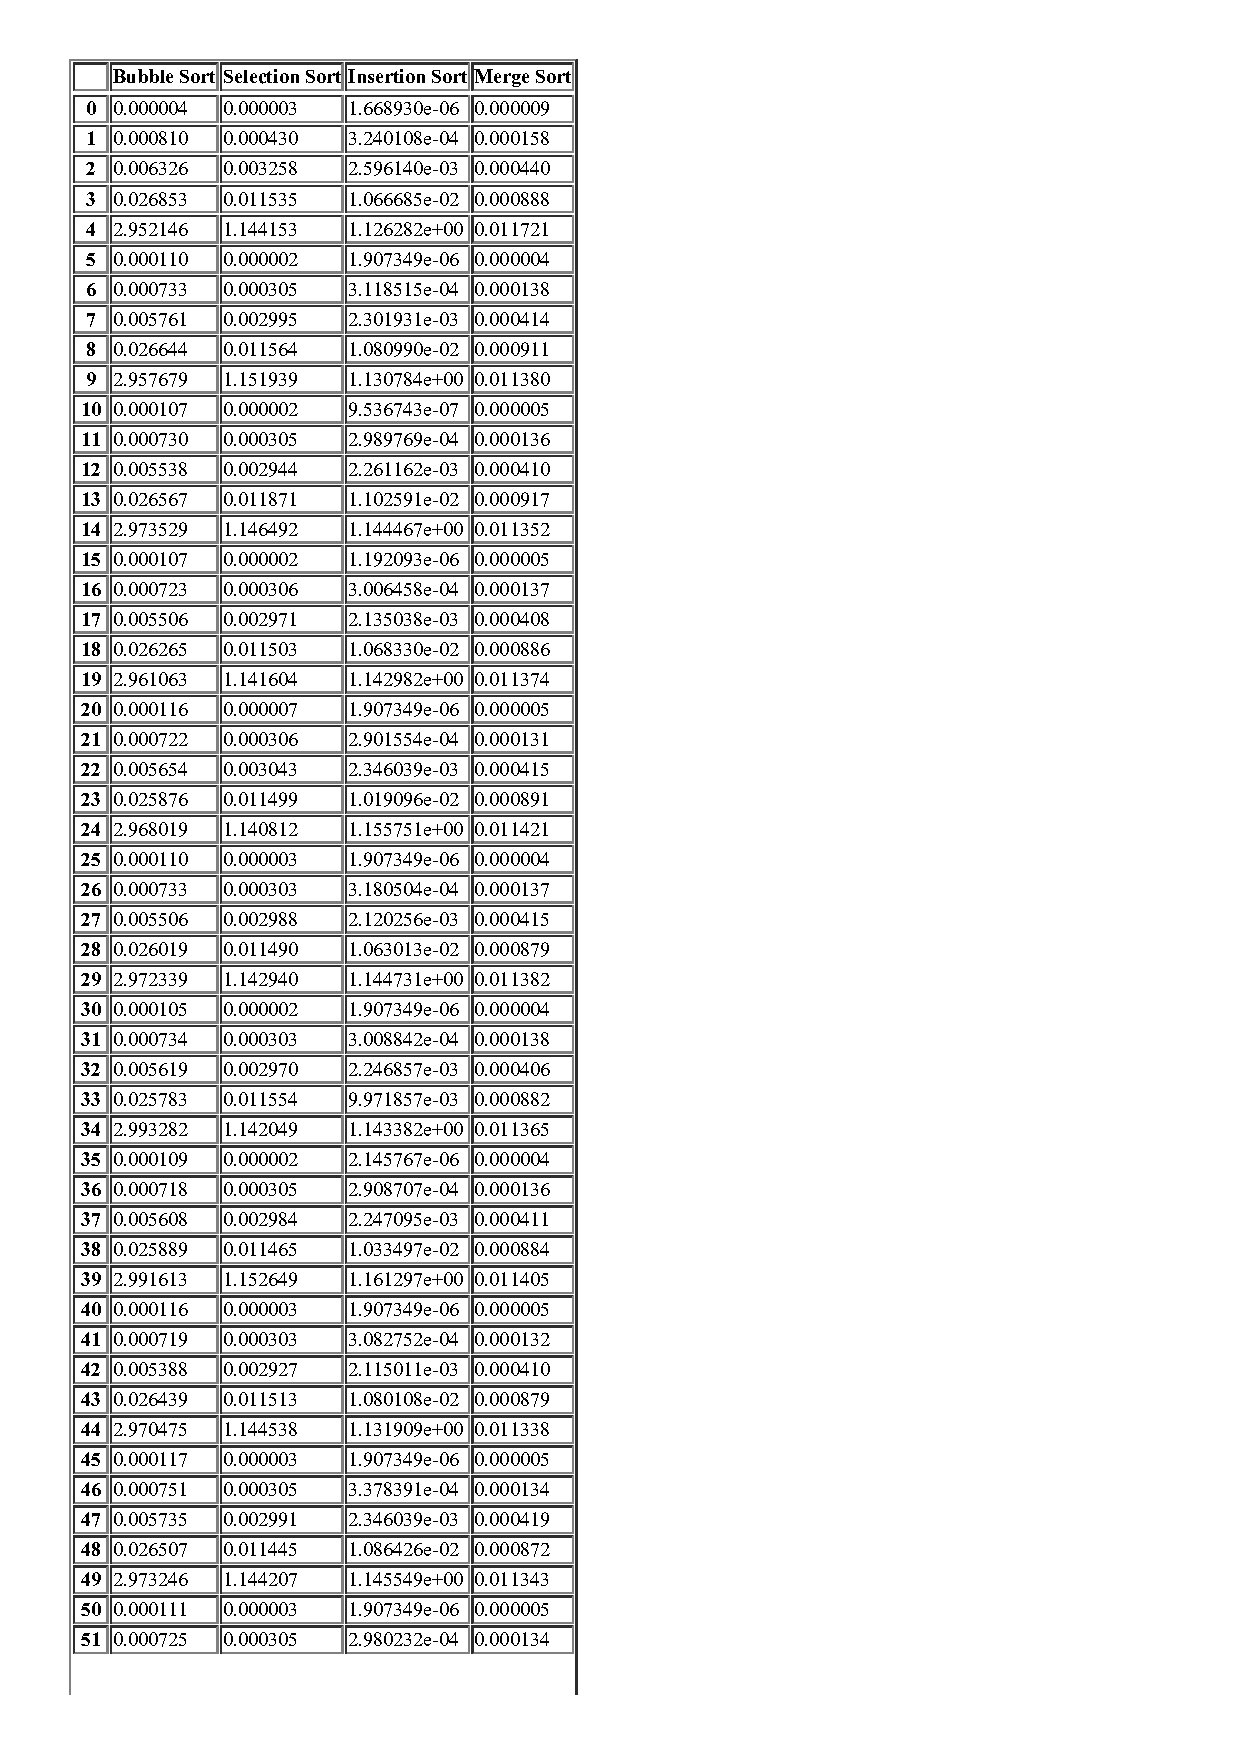
\includepdf[pages=-]{SortingTests.pdf}

\end{document}
